\documentclass[tikz]{standalone}
\usepackage{tikz}
\usetikzlibrary{arrows.meta,positioning,shapes.geometric,shapes.misc,fit,backgrounds,calc,decorations.pathreplacing}

\definecolor{cEmpirical}{HTML}{2B7A78}
\definecolor{cConjectured}{HTML}{C07C38}
\definecolor{cSpeculative}{HTML}{A04050}
\definecolor{cLimit}{HTML}{6B5CA5}

\begin{document}
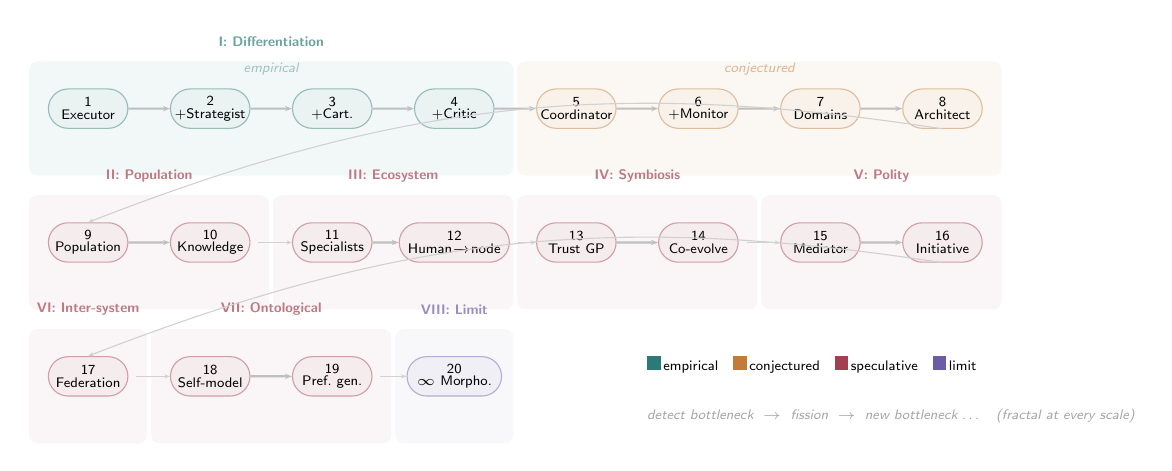
\begin{tikzpicture}[
    phase/.style={rounded rectangle, draw=#1!50, fill=#1!10, minimum width=1.15cm, minimum height=0.5cm, font=\fontsize{4.5}{5.5}\selectfont\sffamily, inner sep=2pt, align=center},
    epoch/.style={font=\fontsize{5}{6}\selectfont\sffamily\bfseries, text=black!60},
    arr/.style={-{Stealth[length=2.5pt]}, thick, black!25},
    earr/.style={-{Stealth[length=2pt]}, black!18, thin},
    every node/.style={align=center}
]

\def\xs{1.55}  % x spacing

% ============================================================
% Row 1: Epoch I — Differentiation (Phases 1–8)
% ============================================================

\begin{scope}[on background layer]
    \fill[cEmpirical!6, rounded corners=3pt] (-0.75, 0.6) rectangle (3*\xs+0.75, -0.85);
    \fill[cConjectured!6, rounded corners=3pt] (4*\xs-0.75, 0.6) rectangle (7*\xs+0.75, -0.85);
\end{scope}

\node[phase=cEmpirical] (p1) at (0, 0) {1\\[-1pt]Executor};
\node[phase=cEmpirical] (p2) at (\xs, 0) {2\\[-1pt]+Strategist};
\node[phase=cEmpirical] (p3) at (2*\xs, 0) {3\\[-1pt]+Cart.};
\node[phase=cEmpirical] (p4) at (3*\xs, 0) {4\\[-1pt]+Critic};
\node[phase=cConjectured] (p5) at (4*\xs, 0) {5\\[-1pt]Coordinator};
\node[phase=cConjectured] (p6) at (5*\xs, 0) {6\\[-1pt]+Monitor};
\node[phase=cConjectured] (p7) at (6*\xs, 0) {7\\[-1pt]Domains};
\node[phase=cConjectured] (p8) at (7*\xs, 0) {8\\[-1pt]Architect};

\foreach \i/\j in {1/2,2/3,3/4,4/5,5/6,6/7,7/8} { \draw[arr] (p\i) -- (p\j); }

\node[epoch, text=cEmpirical!70] at (1.5*\xs, 0.85) {I: Differentiation};
\node[font=\fontsize{3.5}{4}\selectfont\sffamily\itshape, text=cEmpirical!45] at (1.5*\xs, 0.5) {empirical};
\node[font=\fontsize{3.5}{4}\selectfont\sffamily\itshape, text=cConjectured!55] at (5.5*\xs, 0.5) {conjectured};

% ============================================================
% Row 2: Epochs II–IV (Phases 9–14)
% ============================================================

\def\ry{-1.7}

% Epoch II
\begin{scope}[on background layer]
    \fill[cSpeculative!5, rounded corners=3pt] (-0.75, \ry+0.6) rectangle (\xs+0.75, \ry-0.85);
\end{scope}
\node[phase=cSpeculative] (p9) at (0, \ry) {9\\[-1pt]Population};
\node[phase=cSpeculative] (p10) at (\xs, \ry) {10\\[-1pt]Knowledge};
\draw[arr] (p9) -- (p10);
\node[epoch, text=cSpeculative!70] at (0.5*\xs, \ry+0.85) {II: Population};

% Epoch III
\begin{scope}[on background layer]
    \fill[cSpeculative!5, rounded corners=3pt] (2*\xs-0.75, \ry+0.6) rectangle (3*\xs+0.75, \ry-0.85);
\end{scope}
\node[phase=cSpeculative] (p11) at (2*\xs, \ry) {11\\[-1pt]Specialists};
\node[phase=cSpeculative] (p12) at (3*\xs, \ry) {12\\[-1pt]Human$\to$node};
\draw[arr] (p11) -- (p12);
\node[epoch, text=cSpeculative!70] at (2.5*\xs, \ry+0.85) {III: Ecosystem};

% Epoch IV
\begin{scope}[on background layer]
    \fill[cSpeculative!5, rounded corners=3pt] (4*\xs-0.75, \ry+0.6) rectangle (5*\xs+0.75, \ry-0.85);
\end{scope}
\node[phase=cSpeculative] (p13) at (4*\xs, \ry) {13\\[-1pt]Trust GP};
\node[phase=cSpeculative] (p14) at (5*\xs, \ry) {14\\[-1pt]Co-evolve};
\draw[arr] (p13) -- (p14);
\node[epoch, text=cSpeculative!70] at (4.5*\xs, \ry+0.85) {IV: Symbiosis};

% Row 2 continued: Epochs V–VIII

% Epoch V
\begin{scope}[on background layer]
    \fill[cSpeculative!5, rounded corners=3pt] (6*\xs-0.75, \ry+0.6) rectangle (7*\xs+0.75, \ry-0.85);
\end{scope}
\node[phase=cSpeculative] (p15) at (6*\xs, \ry) {15\\[-1pt]Mediator};
\node[phase=cSpeculative] (p16) at (7*\xs, \ry) {16\\[-1pt]Initiative};
\draw[arr] (p15) -- (p16);
\node[epoch, text=cSpeculative!70] at (6.5*\xs, \ry+0.85) {V: Polity};

% ============================================================
% Row 3: Epochs VI–VIII (Phases 17–20)
% ============================================================

\def\rry{-3.4}

% Epoch VI
\begin{scope}[on background layer]
    \fill[cSpeculative!5, rounded corners=3pt] (-0.75, \rry+0.6) rectangle (0.75, \rry-0.85);
\end{scope}
\node[phase=cSpeculative] (p17) at (0, \rry) {17\\[-1pt]Federation};
\node[epoch, text=cSpeculative!70] at (0, \rry+0.85) {VI: Inter-system};

% Epoch VII
\begin{scope}[on background layer]
    \fill[cSpeculative!5, rounded corners=3pt] (\xs-0.75, \rry+0.6) rectangle (2*\xs+0.75, \rry-0.85);
\end{scope}
\node[phase=cSpeculative] (p18) at (\xs, \rry) {18\\[-1pt]Self-model};
\node[phase=cSpeculative] (p19) at (2*\xs, \rry) {19\\[-1pt]Pref.\ gen.};
\draw[arr] (p18) -- (p19);
\node[epoch, text=cSpeculative!70] at (1.5*\xs, \rry+0.85) {VII: Ontological};

% Epoch VIII — The Limit
\begin{scope}[on background layer]
    \fill[cLimit!5, rounded corners=3pt] (3*\xs-0.75, \rry+0.6) rectangle (3*\xs+0.75, \rry-0.85);
\end{scope}
\node[phase=cLimit] (p20) at (3*\xs, \rry) {20\\[-1pt]$\infty$ Morpho.};
\node[epoch, text=cLimit!70] at (3*\xs, \rry+0.85) {VIII: Limit};

% ============================================================
% Inter-row transitions
% ============================================================

% Row 1 → Row 2
\draw[earr, bend right=15] (p8.south) to (p9.north);
\draw[earr] (p10.east) ++(0.1,0) -- (p11.west);
\draw[earr] (p12.east) ++(0.1,0) -- (p13.west);
\draw[earr] (p14.east) ++(0.1,0) -- (p15.west);

% Row 2 → Row 3
\draw[earr, bend right=15] (p16.south) to (p17.north);
\draw[earr] (p17.east) ++(0.1,0) -- (p18.west);
\draw[earr] (p19.east) ++(0.1,0) -- (p20.west);

% ============================================================
% Annotations
% ============================================================

% Self-similarity note
\node[font=\fontsize{4}{5}\selectfont\sffamily\itshape, text=black!35, anchor=west] at (4.5*\xs, \rry-0.5)
    {detect bottleneck\; $\to$\; fission\; $\to$\; new bottleneck\;\ldots\quad(fractal at every scale)};

% Epistemic legend
\node[font=\fontsize{4}{5}\selectfont\sffamily, anchor=west] at (4.5*\xs, \rry+0.15) {%
    \textcolor{cEmpirical}{\rule{5pt}{5pt}}\,empirical\quad
    \textcolor{cConjectured}{\rule{5pt}{5pt}}\,conjectured\quad
    \textcolor{cSpeculative}{\rule{5pt}{5pt}}\,speculative\quad
    \textcolor{cLimit}{\rule{5pt}{5pt}}\,limit%
};

\end{tikzpicture}
\end{document}
